\section{Data and Institutional Context} \label{chap:data}
\subsection{Institutional Context}
Western Germany has a long tradition of collective bargaining systems, which kept wages relatively high until the 90's. However, the reunification with  deindustrialised Eastern Germany and the Hartz labor market reforms of 2003 strongly reduced industry compliance, dropping coverage rates from a near universal 85\% in 1990 to barely 60\% in 2013 (and not even 50\% in the East) \citep{Weinkopf2015}. Trade unions, which initially favoured sector-level agreements, started pushing for a national minimum wage, but met heavy political resistance. At the time, Germany was still considered the \emph{sick man of Europe}, with unemployment rates above 10\%, only turning into an economic superstar from 2008 onwards \citep{Dustmann2014}. The surge in economic prowess also led to increased support for a national minimum wage, as rising GDP failed to lift wages for the bottom deciles.

The Social Democratic Party of Germany (SPD) forced the issue in 2013 by making their entry in the governing coalition conditional on the introduction of a national minimum wage \citep{Weinkopf2015}. The Minimum Wage Act went into force on January 1st 2015, setting a national wage floor of €8.50 (then \$11.05) and strengthening collective agreements (exceeding the national minimum). There are only very few exceptions - mainly interns (in a clear educational context), minors, trainees, volunteers and previously long-term unemployed during their first six months in a new job. Additionally, certain sectors (e.g. meat processing, hair dressing) were allowed a two year transition period. We exclude those from our analysis. 

% Replication: ctrl+F #mwtomedianwageGraph
\begin{figure}[htb]
    \centering
    \caption{Ratio of Minimum Wage to Median Wage}
    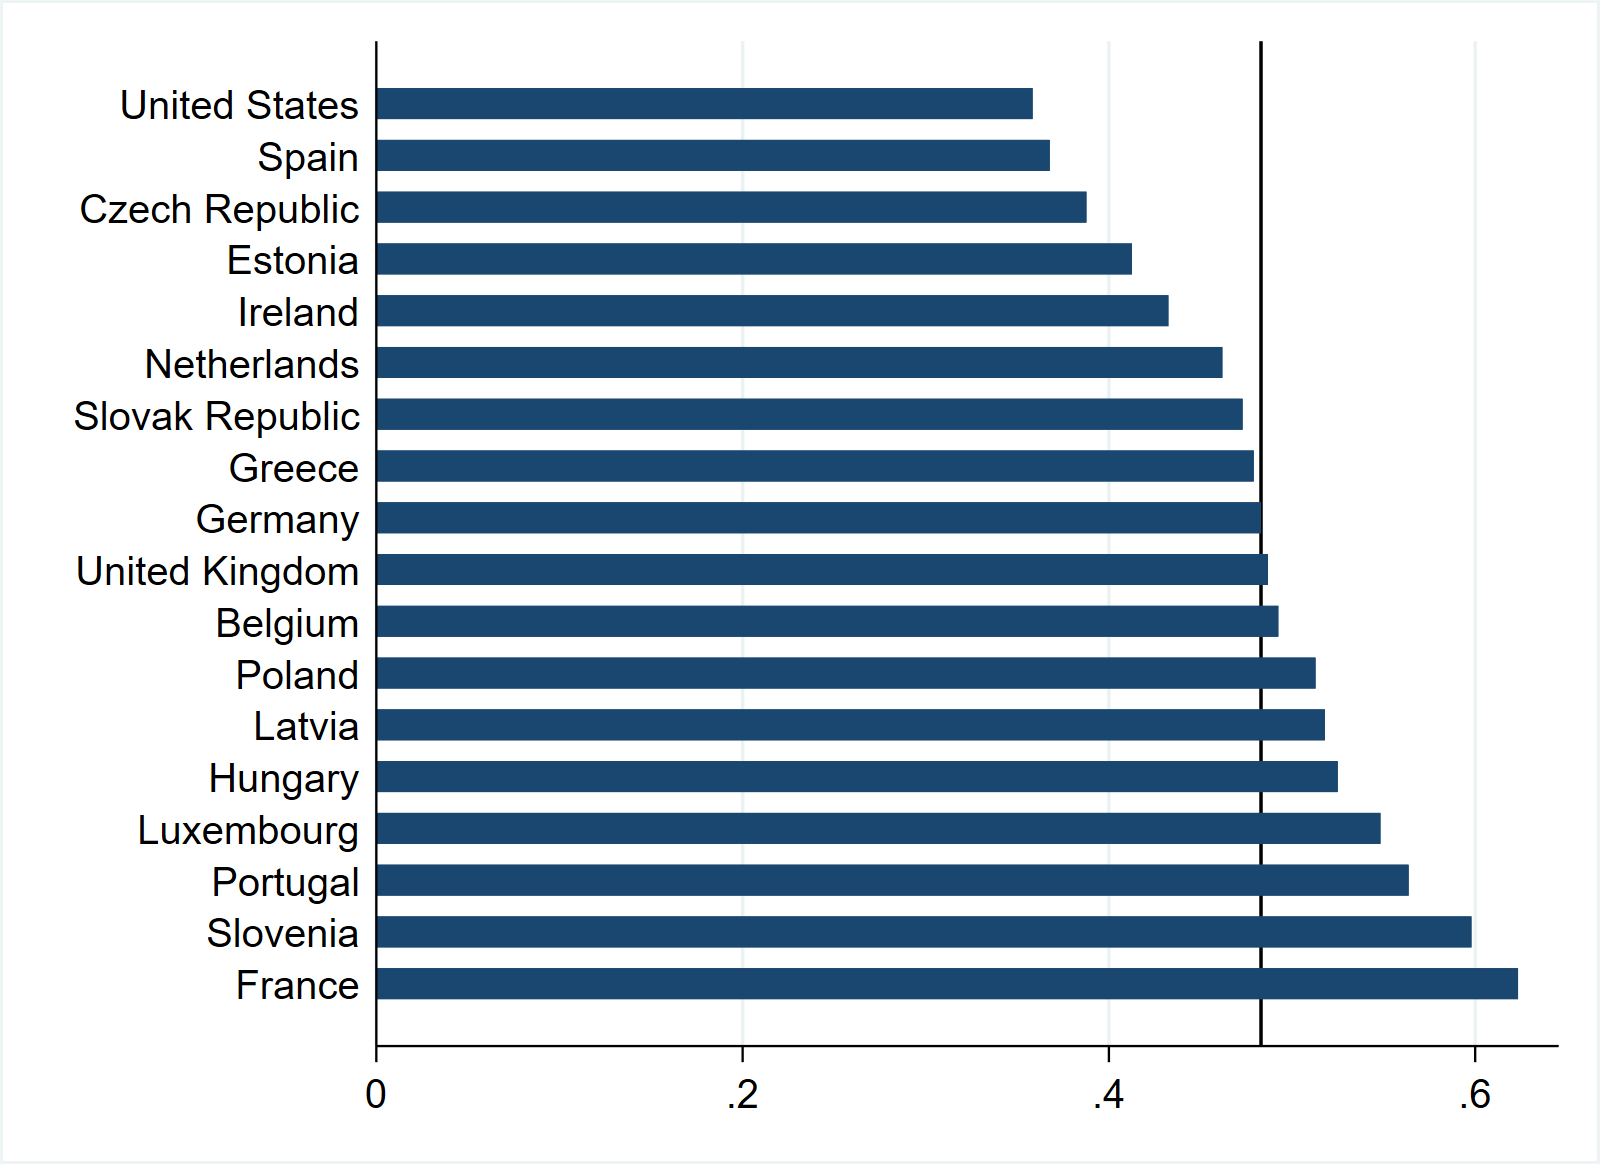
\includegraphics[width=0.60\paperwidth]{Images/mwToMedianWage.png}
    \label{fig:mwtomedian}
    \caption*{Source: \citet{OECDmw}}
\end{figure}

Figure \ref{fig:mwtomedian} shows Germany's National Minimum Wage (NMW) is set at a similar (relative) level as those present in other countries. About 2.8 million eligible employees earned less than €8.50 per hour in 2014 (11\%, \citet{Burauel2017}), albeit with sizeable differences across sectors and regions (Figure \ref{fig:correlationIndicators} in the Appendix). Own back of the envelope calculations based on the SOEP suggest that on average they would require a raise of €2.41/hr to comply with the NMW. Full compliance would raise the total wage bill by 2\%.

The minimum wage commission decides on the future evolution of the policy and consists of voting representatives from industry (3), unions (3) and two advisory members from the academic community. This led to a first increase in 2017, when the minimum wage was raised from €8.50 to €8.84, suggesting the minimum wage will be raised gradually (the 2017 hike amounts to a 4\% increase), rather than in larger discrete jumps as is more customary in the US.\footnote{The average size of minimum wage changes in the US between 1990-2013 was 9.5\% \citep{Wursten2017}.}

\subsection{Firm-level Data}
The core of this study is the Mannheim Enterprise Panel (MUP) hosted by the Centre for Economic Research (ZEW). It is based on data obtained from Creditreform, the largest creditrating agency in Germany and covers all German corporations \citep{Steven2017}. The dataset is representative for the German economy and can thus be used to formulate population-level conclusions \citep{Bersch2014}. The main variables of interest are employment and turnover, but also the assigned creditratings. These are based on a combination of public and private sources, e.g. public trade registers and court filings as well as private data on payment reliability and even manager interviews. As a result, these ratings contain more information on a firm's health than traditional balance sheet items. We drop outliers based on changes in the creditrating and employment or turnover (depending on the dependent variable) to retain the largest and smallest firms but still filter out input errors as well as massive swings due to mergers and acquisitions.

\subsection{Sector-level Treatment Indicator}
Our identification strategy is based on comparing firms in heavily affected sectors to similar counterparts in largely unaffected sectors. In order to construct this `vulnerability' indicator, we turn to the German Socio-Economic Panel (SOEP version 32), a yearly survey of private households which has been conducted since 1984 in West Germany and since 1990 in East Germany (comparable to the Current Population Survey in the US). Crucially, it contains monthly wages as well as hours worked information, which we combine to obtain an estimate of each individual's hourly wage. Restricting our sample to eligible persons in 2013-2014 (right before the introduction of the minimum wage), we can then calculate for each two-digit sector how many employees were earning less than the NMW.\footnote{We use the Nace Rev 2 classification, which is based on the international ISIC standard and can fairly easily be compared to the US NAICS system.} Given the substantial wage differences between East and West Germany, we further split this across the two parts. 

Table \ref{table:sectorBite} provides an overview of the most and least affected sectors. As in the US, we see that the restaurant and fastfood sector (Nace 56) is most heavily affected. Unaffected sectors are for example waste collection, financial services and the higher value manufacturing sectors. The table also shows the average gap between the sub-NMW earners' wage in 2014 and the NMW and how much that sector's total wage bill would rise under full compliance (and no other wage movement).

We use the share of sub-NMW workers to split the industries into three groups: treated, grey zone and controls, for East and West Germany separately given their economic differences. Any sector where this share exceeds 30\% is defined as treated, below 10\% is considered control. Those in between we consider to be in the grey zone and exclude from the analysis. Table \ref{table:sectorOverview} shows the treatment allocation per sector-region (region: East or West Germany), as well as the distribution of firms in our regression sample over sector-regions. The differences between East and West Germany are remarkably stark. Only the food and beverages sector (`restaurants') and accommodation sectors are treated in the West, whereas only seven sectors qualify as controls in the East. Conversely, there are 29 treated sectors in the East, whereas the West has 27 control sectors. 

% Replication: ctrl+F #sectorOverviewTable
\begin{table}[htbp]\centering
\setlength\tabcolsep{3pt}
\small
\caption{Treated, Untreated and Greyzone Sectors}\label{table:sectorOverview}
\begin{threeparttable}
    \begin{tabular}{r|c|c|l}
    \toprule
Nace & Treatment & \# of firms & Nace  \\
Code & West-East & West-East & Text\\
\midrule
56&	T-T&	1018 - 124&	Food and beverage service activities\\
55&	T-T&	626 - 158&	Accommodation\\
\midrule
47&	GZ-T&	9149 - 1255&	Retail trade, excl. of motor vehicles and motorcycles\\
70&	GZ-T&	6270 - 313&	Activities of head offices; management consultancy activities\\
45&	GZ-T&	4646 - 1017&	Wholesale and retail trade and repair of motor vehicles and motorcycles\\
68&	GZ-T&	4066 - 605&	Real estate activities\\
71&	GZ-T&	2702 - 454&	Architectural and engineering activities; technical testing and analysis\\
52&	GZ-T&	2021 - 309&	Warehousing and support activities for transportation\\
82&	GZ-T&	1670 - 169&	Admin, office support and other business support activities\\
66&	GZ-T&	1509 - 160&	Activities auxiliary to financial services and insurance activities\\
10&	GZ-T&	1233 - 257&	Manufacture of food products\\
77&	GZ-T&	968 - 236&	Rental and leasing activities\\
23&	GZ-T&	881 - 202&	Manufacture of other non-metallic mineral products\\
73&	GZ-T&	987 - 68&	Advertising and market research\\
69&	GZ-T&	874 - 99&	Legal and accounting activities\\
79&	GZ-T&	763 - 81&	Travel agency, tour operator and related activities\\
74&	GZ-T&	746 - 51&	Other professional, scientific and technical activities\\
31&	GZ-T&	625 - 89&	Manufacture of furniture\\
93&	GZ-T&	506 - 65&	Sports activities and amusement and recreation activities\\
13&	GZ-T&	352 - 72&	Manufacture of textiles\\
78&	GZ-T&	317 - 31&	Employment activities\\
11&	GZ-T&	272 - 29&	Manufacture of beverages\\
95&	GZ-T&	215 - 44&	Repair of computers and personal and household goods\\
14&	GZ-T&	171 - 18&	Manufacture of wearing apparel\\
80&	GZ-T&	130 - 21&	Security and investigation activities\\
63&	GZ-T&	118 - 8&	Information service activities\\
15&	GZ-T&	68 - 10&	Manufacture of leather and related products\\
50&	GZ-T&	53 - 5&	Water transport\\
12&	GZ-T&	11 - 1&	Manufacture of tobacco products\\
\midrule
64&	C-C&	956 - 51&	Financial service activities, excl. insurance and pension funding\\
38&	C-C&	608 - 219&	Waste collection, treatment and disposal activities; materials recovery\\
35&	C-C&	652 - 167&	Electricity, gas, steam and air conditioning supply\\
37&	C-C&	108 - 34&	Sewerage\\
84&	C-C&	106 - 18&	Public administration and defence; compulsory social security\\
39&	C-C&	37 - 4&	Remediation activities and other waste management services\\
\midrule
43&	C-GZ&	15765 - 3844&	Specialised construction activities\\
25&	C-GZ&	4969 - 964&	Manufacture of fabricated metal products, excl. machinery and equipment\\
41&	C-GZ&	3159 - 772&	Construction of buildings\\
28&	C-GZ&	3102 - 392&	Manufacture of machinery and equipment n.e.c.\\
62&	C-GZ&	2603 - 250&	Computer programming, consultancy and related activities\\
26&	C-GZ&	1180 - 170&	Manufacture of computer, electronic and optical products\\
42&	C-GZ&	796 - 297&	Civil engineering\\
27&	C-GZ&	898 - 144&	Manufacture of electrical equipment\\
32&	C-GZ&	834 - 110&	Other manufacturing\\
20&	C-GZ&	594 - 86&	Manufacture of chemicals and chemical products\\
85&	GZ-C&	536 - 95&	Education\\
33&	C-GZ&	464 - 124&	Repair and installation of machinery and equipment\\
24&	C-GZ&	498 - 71&	Manufacture of basic metals\\
29&	C-GZ&	339 - 68&	Manufacture of motor vehicles, trailers and semi-trailers\\
17&	C-GZ&	329 - 49&	Manufacture of paper and paper products\\
30&	C-GZ&	135 - 32&	Manufacture of other transport equipment\\
21&	C-GZ&	124 - 19&	Manufacture of basic pharmaceutical products and preparations\\
65&	C-GZ&	105 - 4&	(re-)Insurance and pension funding, excl. compulsory social security\\
36&	C-GZ&	36 - 21&	Water collection, treatment and supply\\
51&	C-GZ&	18 - 0&	Air transport\\
9&	C-GZ&	6 - 3&	Mining support service activities\\
6&	C-GZ&	3 - 0&	Extraction of crude petroleum and natural gas\\
    \bottomrule
    \end{tabular}
\begin{tablenotes}
\item \footnotesize T: treated, C: control, GZ: grey zone (excluded). Table sorted by treatment status and number of firms in the sector. Unlisted sectors are a) in grey zone in both areas, b) excluded based on legislative reasons or c) excluded due to pre-existing higher sectoral minimum wage agreements.
\end{tablenotes}
\end{threeparttable}
\end{table}